\documentclass[11pt]{article}
\usepackage{geometry} % see geometry.pdf on how to lay out the page. There's lots.
\usepackage{hyperref}
\usepackage{graphicx}
\usepackage{gensymb}
\usepackage[affil-it]{authblk}
\usepackage[toc,page]{appendix}
\usepackage{pifont}
\usepackage{amsmath}
\usepackage{amssymb}
\usepackage{relsize}
\usepackage{draftwatermark}
\usepackage[mathscr]{eucal}
\usepackage{amsmath, amssymb, graphics, setspace}

\newcommand{\mathsym}[1]{{}}
\newcommand{\unicode}[1]{{}}

\SetWatermarkText{DRAFT}
\SetWatermarkScale{6}
\SetWatermarkLightness{0.95}

\DeclareMathOperator{\atantwo}{atan2}
\DeclareMathOperator{\sign}{sign}
\DeclareMathOperator{\sense}{sense}

% \geometry{letter} % or letter or a5paper or ... etc
% \geometry{landscape} % rotated page geometry

% See the ``Article customise'' template for come common customisations

\title{Numerical Optimization of Tetrahelical Robots via Derivatives}
\author{Robert L. Read
  \thanks{read.robert@gmail.com}
}
\affil{Founder, Public Invention, an educational non-profit.}


\date{\today}

%%% BEGIN DOCUMENT
\begin{document}

\maketitle

%% \tableofcontents

\section{Introduction}

A {\em variable geometry truss} is a truss in which changes shape by means of the change of the length of members, in contrast
to many robot arms which change joint angles. We call a member which can change length an {\em actuator}.
A truss constructed purely by starting with a triangle and repeatedly adding two members and a new joint to one side of an existing triangle
to form a new triangle is a {\em simple truss}. This paper
is concerned only with simple planar trusses. In particular, we focus on trusses isomorphic to the Warren truss (e.g., an unbranching configuration of triangles.)
Furthermore, although the world {\em truss} connotes forces and structural analysis,
we are concerned purely with geometry. Although motivated by robotics, we assume that our trusses and actuators are strong enough that
we need not consider the forces acting upon the truss---in other words, we are treating it as mechanism and not a machine.

If we imagine a joint, usually at one end of our truss, to be an end effector, 
the fundamental goal of this paper is to answer the question:
\begin{quote}
  How does a change in length of an actuator change the position of an end effector?
\end{quote}

\section{Formulation}

A {\em truss} structure is a graph and a set of fixed nodes $T=(G,F)$. $G = (V,E)$. $V$ is a set of nodes or joints. $E$ is a set of lines or members which are 2-element subsets of $V$.
At least two nodes are considered to be fixed in space via a set of fixed nodes $F = {(i,x,y) \| i \in V \and x,y \in \mathbb{R}}$.

We number joints from zero and designate them with a subscript. Members are designated by two subscripts, naming the joints they connect.

A {\em configuration} is a function mapping each member of a truss structure to a non-negative length. $C: V \times V \mapsto \mathbb{R}$.

A {\em geometry} is a placement of each joint in the Cartesian plane. $G: V \mapsto \mathbb{R} \times \mathbb{R} $.

A {\em simple truss} is a truss constructed from a triangle by adding a single joint and two members to a side repetitively.
A {\em Warren truss} is an unbranched simple truss, which is isomorphic to a truss that is a single chain of equilateral triangles.
Furthermore, we insist that each even node $n$ occurs as a anti-clockwise turn (in the anti-clockwise semiplane) from the vector $\overrightarrow{n-2,n-1}$, and
each odd node occurs as a clockwise turn (in the clockwise semiplane) from the previous to nodes.

For a Warren truss, there is a simple algorithm $W$ for computing a geometry from a configuration: $W : C \mapsto G$.

A goal joint is a joint $j$ such that $j \in V$ and a desired position given by a goal function $d : V \mapsto \mathbb{R}^2$. In robotics,
a goal joint is often called an {\em end effector}.

A {\em scoring function} is a function that that takes a geometry and returns a real, non-negative value based on 
the goal node positions given by by a goal function and the actual position given by a Geometry. A score of zero is considered
 a perfect score and the a higher score represents a less sought-after result.

A {\em linear distance scoring function} is a special scoring function that that takes a geometry and returns a real, non-negative value based solely
on a summation of distances between the goal node positions given by by a goal function and the actual position given by a Geometry.

A truss {\em problem} $P = (T,d,s)$ is a truss with a scoring function and a desired position function.
A solution to a problem is a configuration and a geometry. An optimal solution is a solution which minimizes the score.

Our fundamental goal is to develop a formula for the partial derivative of the end effector
with respect to the change in length of a member.

A further goal is to be able to render a diagram illustrating the impact on the end-effector
of a change of each member, as drawn by rendering a vector from the center point of each member.

A further goal is to have algorithms to determine:
\begin{itemize}
\item What is the minimum overall change in length to a group of actuators to solve a Problem?
\item Can a Problem be solved with a single change in length?
\item Assuming bounds on the lengths of actuators, can we solve Problems?
  \item What is the workspace of a truss?
  \end{itemize}

In the remainder of this paper we will consider only Warren trusses, linear distance scoring functions, and desired position functions
that map only one node, called an end effector, to a desired position. Furthermore, we will assume that the first two nodes are fixed
and that the furthest node (by path length) from the first node is the end effector.

\section{Moving an External Member}

We seek a formula for the change in position of the end effector $e$ with respect to change in the length of a member given a geometry.
In the case of a Warren truss, all members can be divided between external members and internal members. A change to the length of an
external member is particularly simple.

The change in position is a centered on the goal node representing the place the goal node would move to with a unit change in length.
However, the derivative is only valid as an infinitessimal, but as an infinitessimal its magnitude and direction may be usefully
added to or compared to other such vectors. We can thus usefully tell which member would change the position of the goal node most
rapidly in response to a minute change in different members.

\begin{figure}
  \centering
  \includegraphics[width=\textwidth]{External_angle_Change.png}
  \caption{A Trusss Problem with Change to an External Member Length}  
\end{figure}

The fundamental observation is that for an external member $(C,A)$, a change in length generates a rotation $\theta$ about joint $B$
whose position is given by $(B_x,B_y)$. $\theta$ is the angle of the vector from the pivot point $B$ to the end-effector $E$ with the $x$-axis.
This rotation applies to the triangle defined by three joints: $\triangle B,C,E$. Not that this triangle doeS not exist as a physical
structure in the truss. 

By using the law of cosines, where $a = \|\overrightarrow{A,B}\|, b = \|\overrightarrow{A,C}\|, c = \|\overrightarrow{B,C}\| $,
where $b$ is the member opposite the pivot joint $B$ which changes the angle $ \phi_{i-1} = \angle ABC $. In other words, $\phi$ is a signed angle measure
$BA$ moved into $BC$, with positive representing anti-clockwise.
\[
\cos{\phi} = \frac{a^2 - b^2 + c^2}{2 a c}
\]
or
\[
\phi = \arccos{\frac{a^2 - b^2 + c^2}{2 a c}}
\]
Using Woflram Alpha to differentiate this, we obtain:

\[
\frac{\partial \phi}{\partial b} = \frac{b}{ac\sqrt{1 - \frac{(a^2 + c^2 - b^2)^2}{4a^2c^2}}}
\]

This derivation loses the sign information, which we recover by considering whether $S = \sign{\phi}$.

The change in the end effector is always perpendicular to the drawn from the pivot joint to the effector and proportional to its length.
An alternative way of looking at this is that the result should be orthogonal to the vector
\[
\begin{bmatrix}
           (e_x  - x) \\
           (e_y - y)  \\
\end{bmatrix}
\]
In other words:
\[
S \cdot
\begin{bmatrix}
           - (e_y  - y) \\
           (e_x - x)  \\
\end{bmatrix}
\]
With the sign $S$ is negative if $\phi$ is clockwise. $\phi$ cannot be zero or equal or exceed $\pi$ in a physical machine is excluded for that reason.

Since the change in $\phi$ is equal to the change in $\theta$, we can use the chain rule:

\[
\frac{\partial e}{\partial  b} = \begin{bmatrix}
           \frac{\partial e_x}{\partial b} \\
           \frac{\partial e_y}{\partial b} \\
         \end{bmatrix} = \frac{Sb}{ac\sqrt{1 - \frac{(a^2 + c^2 - b^2)^2}{4a^2c^2}}} \begin{bmatrix}
           -(e_y -y)  \\
           (e_x - x )  \\
         \end{bmatrix}
\]

So this is a closed-form expression for the change in the position of an end effector for any external member $i,i-2$ we choose. If we then know how the
scoring functions changes as the end effector moves, we can compute the change in the scoring functions as we change $b = \| AC \|$, which is what
we need for numeric optimization.

\section{Moving an Internal Member}


In the Internal Member Length change diagram, $\angle ABC = \beta $, $\angle CBD = \psi$, $\angle BCD = \chi$,
$\angle ACB = \gamma$, $\angle BDC = \delta$, and $\angle BAC = \alpha$. The lengths are marked $a,b,c,f,g$, with $a$ being opposite node $A$ and a diagonal
of the quadrilateral $ABDC$.




Furthermore, $\angle ABD = \beta + \psi$, and $\angle ACD = \gamma + \chi$.

The absolute angle between the line between the fixed nodes $A$ and $B$ and the $x$-axis is $\rho$ (counting positive as anticlockwise from the $x$-axis.)
Both $A$ and $B$ are considered fixed, but both $C$ and $D$ move as $a$ changes. $D$ rotates about $B$ and $C$ rotatest about $A$.

\begin{figure}
  \centering
  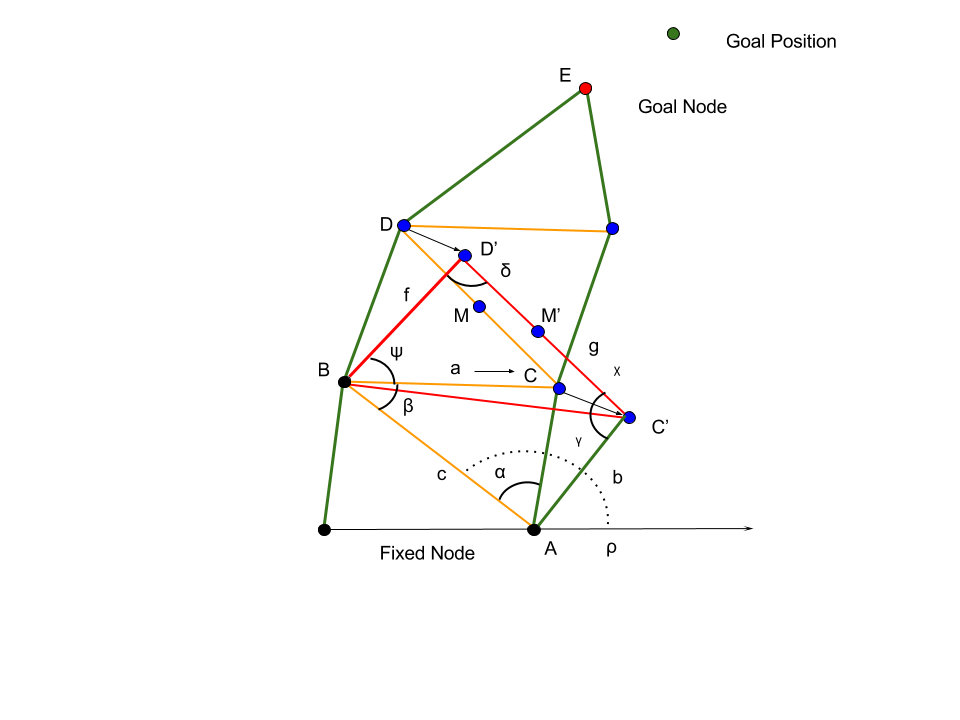
\includegraphics[width=0.7\textwidth]{Internal_angle_change.png}
  \caption{A Trusss Problem with Change to an Internal Member Length}  
\end{figure}


Because the member $DC$ does not change its length, we conceptualize the impact of a change to length $a$ as translating  between $C$ and $D$ and
rotating $BC$ about $M$. By knowing the change in the absolute rotation and the change in the position of $M$ as $a$ changes infintessimally, we know how the
end effector $E$ changes.


We can compute $\frac{\partial \beta}{\partial a}$ directly (using Wolfram Alpha) from $\phi$:
\[
\beta = \arccos{\frac{a^2 - b^2 + c^2}{2 a c}}
\]

\[
\frac{\partial \beta}{\partial a} =
-\frac{\frac{1}{c} - \frac{a^2 - b^2 + c^2}{2 a^2 c}}
{\sqrt{1 - \frac{(a^2 - b^2 + c^2)^2}{4 a^2 c^2}}}
\]

Calculating the same way for $\alpha$ in order to have $C$
\[
\alpha = \arccos{\frac{-a^2 +  b^2 + c^2}{2 b c}}
\]

\[
\frac{\partial \alpha}{\partial a} =
\frac{a}
{bc \sqrt{1 - \frac{(-a^2 + b^2 + c^2)^2}{4 b^2 c^2}}}
\]

\[ \gamma = \pi - (\alpha + \beta) \]

Now we compute $\chi$ from the law of cosines:
\[
\chi = \arccos{\frac{a^2 - f^2 + g^2}{2 a g}}
\]

\[
\frac{\partial \chi}{\partial a} =
-\frac{\frac{1}{g} - \frac{a^2 - f^2 + g^2}{2 a^2 g}}
{\sqrt{1 - \frac{(a^2 - f^2 + g^2)^2}{4 a^2 g^2}}}
\]


\[
\begin{bmatrix}
  C_x \\
  C_y \\
\end{bmatrix} =
\begin{bmatrix}
 A_x + b \cos{(\rho - \alpha)} \\
 A_y + b \sin{(\rho - \alpha)} \\
\end{bmatrix}
\]

Taking the derivative of this with respect to $a$,

\[
\begin{bmatrix}
  \frac{\partial C_x}{\partial a} \\
  \frac{\partial C_y}{\partial a} \\
\end{bmatrix} =
\begin{bmatrix}
 0 + \frac{\partial b \cos{(\rho - \alpha)}}{\partial a} \\
 0 + \frac{\partial b \sin{(\rho - \alpha)}}{\partial a} \\
\end{bmatrix} =
\begin{bmatrix}
b \frac{a\sin{(\rho - \alpha)}}
{bc \sqrt{1 - \frac{(-a^2 + b^2 + c^2)^2}{4 b^2 c^2}}}
  \\
- b \frac{a\cos{(\rho - \alpha)}}
{bc \sqrt{1 - \frac{(-a^2 + b^2 + c^2)^2}{4 b^2 c^2}}}
  \\
\end{bmatrix} =
\frac{a}{c \sqrt{1 - \frac{(-a^2 + b^2 + c^2)^2}{4 b^2 c^2}}}
\begin{bmatrix}
 \sin{(\rho - \alpha)}  \\
- \cos{(\rho - \alpha)}  \\
\end{bmatrix}
\]


The angle $\theta$ between $CD$ and the $x$-axis is therefore given by:
\begin{align*}
  \theta &= \\
  (\rho - \alpha) + (\pi - (\chi + \gamma)) &= \\
\rho + \pi - (\alpha + \chi + (\pi - (\alpha + \beta)) &= \\
\rho + \pi - (\chi + (\pi  -\beta))  &= \\
\rho + -\chi + \beta
\end{align*}
We seek $\frac{\partial \theta}{\partial a}$. However, $\chi$ and $\beta$, computed from $\arccos$,
are ``interanl angles''. We need to seek absolute orientation.

In computing all of this, one must be very careful to keep the signs straight.

In fact, the cleanest way to keep angles straight is to convert angles quickly from ``internal angles'' between two vectors
and compute the ``absolute orientation'' or vectors (that is, the angle measure anticlockwise against the $x$-axis.

The computation of $\frac{\partial \theta}{\partial a}$ above should be considered the computation of an
``absolute orientation''.

We can think of the computation of $\theta = \rho - \chi + \beta$ is a zig zag compuation.
To find the change in the rotation of $\theta$, we find the change in $\chi$ and then the change in $\beta$.

We will say the ``sense'' of an angle $\angle XYZ$  is clockwise or anticlockwise depending on if the
smallest turn from $X$ to $Z$ through $Y$ is clockwise or anitclockwise.

\[
\sense{\angle XYZ} =
\begin{cases}
  0 & \angle XYZ = \pi \\
      1 & \text{ if } \angle XYZ \text{ is anticlockwise moving } \overrightarrow{Y,X} \text{ into } \overrightarrow{Y,Z} \\
      -1 & \text{otherwise}
    \end{cases}
\]

The orientation $\tau = \overrightarrow{B,C}$ is thus $\rho + -(\pi - \|\beta\|)$ if $\angle ABC$ is clockwise,
and $\rho + (\pi - \|\beta\|)$ if $\angle ABC$ is anticlockwsie.

The orientation $\theta = \overrightarrow{C,D}$ is thus $\tau + -(\pi - \|\chi\|)$  if $\angle BCD$ is clockwise,
and $\tau + (\pi - \|\chi\|)$ if $\angle BCD$ is anticlockwise.

\begin{align*}
\theta &= \rho + (\sense{\angle ABC})(\pi - \|\beta\|) + (\sense{\angle BCD})(\pi -\|\chi\|) \\
&= \rho + (\sense{\angle ABC})\pi + (\sense{\angle BCD})\pi +  - (\sense{\angle ABC})\|\beta\|  + - (\sense{\angle BCD})\|\chi\|
\end{align*}

The quantities $\pi$ and $\sense{\angle ABC}$ and $\sense{\angle BCD}$ don't depend on $a$.

\begin{align*}
\frac{\partial \theta}{\partial a} &= 0 + - (\sense{\angle ABC}) \frac{\partial \beta}{\partial a} +
- (\sense{\angle BCD})\frac{\partial \chi}{\partial a}  \\
&= - (\sense{\angle ABC}) \frac{\frac{1}{c} - \frac{a^2 - b^2 + c^2}{2 a^2 c}}
{\sqrt{1 - \frac{(a^2 - b^2 + c^2)^2}{4 a^2 c^2}}}
+ - (\sense{\angle BCD})\frac{\frac{1}{g} - \frac{a^2 - f^2 + g^2}{2 a^2 g}}
{\sqrt{1 - \frac{(a^2 - f^2 + g^2)^2}{4 a^2 g^2}}}
\end{align*}

Now $E$ is simply a translation by $\frac{\partial C}{\partial a}$ by a rotation
about $C$, which as we have previously shown

\[
\frac{\partial e}{\partial  a} = 
\begin{bmatrix}
  \frac{\partial C_x}{\partial a}  \\
  \frac{\partial C_y}{\partial a} \\
  \end{bmatrix}
+
\frac{\partial \theta}{\partial a} 
\begin{bmatrix}
           -(e_y -C_y)  \\
           (e_x - C_x )  \\
         \end{bmatrix}
\]

\[
\frac{\partial e}{\partial  a} =
\frac{a}{c \sqrt{1 - \frac{(-a^2 + b^2 + c^2)^2}{4 b^2 c^2}}}
\begin{bmatrix}
 \sin{(\rho - \alpha)}  \\
- \cos{(\rho - \alpha)}  \\
\end{bmatrix}
+
\frac{\partial \theta}{\partial a} 
\begin{bmatrix}
           -(e_y -C_y)  \\
           (e_x - C_x )  \\
         \end{bmatrix}
\]

\section{Obstacles}

Obstacles may be added to the universe by successfully modifying both the derivative and the objective consistently.

For example, an obstacle may be modelled as a sphere, which provides a positive value for each node which is in the sphere,
and zero for all those not in the sphere.  However, it is better to make this smooth, by for example a polynomial
based on the distance from the center of the sphere.  This allows a derivative to be computed as a direction.
The derivative for a given node will accurately reflect the change in the value of the objective function as moving
toward the the center.

In order to use a gradient-based method with obstacles, we must have a practical way of composing obstacles into the
space of the configuration of the VGT into the objective function, and we must be able to compute an accurate derivative
of the objective function. A naive approach would be to use a flat space which provides a heavy penalty for a node
inside the obstacle. However, it makes more sense to have an objective function which provides directional guidance
to ``push'' a node out of the obstacle. I therefore propose to model an obstacle as disc around a center point and
a radius, with the an increase in the objective function:

\[
\mathcal{O}(\overrightarrow{c},r,\overrightarrow{x}) = \big( \frac{1}{1 + d^2} + 1\big) \cdot \mathcal{H}(r-d)
\]
where $d = \lVert \overrightarrow{c} - \overrightarrow{x} rVert $, and $\mathcal{H}(a,b)$ is the Heaviside step function:

\[
\mathcal{H}(n) =
\begin{cases}
1, & \text{if } n < 0  \\
0, & \text{if } n \geq 0
\end{cases}
\]

The contribution of the obstacle $\mathcal{O}$ to the objective function is:
\[
g(\mathcal{O}(\overrightarrow{c},r,\overrightarrow{x})) = \sum\limits_{n\in G} \mathcal{O}(c,r,\overrightarrow{n})
\]
which allows us to compute the derivative with respect to the change of any member $a$:

\begin{align*}
  \frac{\partial}{\partial a} g(\mathcal{O}(\overrightarrow{c},r,\overrightarrow{x})) &= \frac{\partial}{\partial a} \sum\limits_{n\in G} \mathcal{O}(c,r,\overrightarrow{n}) \\
  &= \sum\limits_{n\in G} \frac{\partial}{\partial a}  \mathcal{O}(c,r,\overrightarrow{n})
\end{align*}
Considering the contribution of a single node $n$:

\begin{align*}
  \frac{\partial}{\partial a}  \mathcal{O}(c,r,\overrightarrow{n}) &=
  \frac{\partial \mathcal{O}(c,r,\overrightarrow{n})}{\partial d(n,c)} \cdot \frac{\partial d(n,c)}{\partial a}
\end{align*}
where:
\begin{align*}
  \frac{\partial d(n,c)}{\partial a} &=  \frac{\partial \overrightarrow{n}}{\partial a} \cdot ({\overrightarrow{n} - \overrightarrow{c}})
\end{align*}
(where $\cdot$ is the inner product.) Note that these two factors are very easy to compute; the previous section gives the formulae
for the change in position of a node with respect to the change in the length of a member ($\frac{\partial \overrightarrow{n}}{\partial a}$).
\begin{align*}  
    \frac{\partial \mathcal{O}(c,r,\overrightarrow{n})}{\partial d(n,c)}  &= \frac{\partial}{\partial d} \big( \frac{1}{(1 + d)^2} + 1\big) \cdot \mathcal{H}(r-d)
\end{align*}

The partical derivative of the Heaviside step function will in fact be discontinous when $r-d = 0$. However,
this is largely irrelevant from a numerical optimization point of view, so long as we can actually compute the
correct derivative. At this (technically unlikely to occur) position we could simply allow the derivative to jump.
If we discover that discontinuity of the derivative is causing a problem, we could use one of several approximations
mentioned by the Wikipedia article \url{https://en.wikipedia.org/wiki/Heaviside_step_function}.

Thanks to Wolfram Alpha, we know this derivative is:
\begin{align*}  
  \frac{\partial \mathcal{O}(c,r,\overrightarrow{n})}{\partial d(n,c)}  &=
  -\big(\frac{1}{(d+1)^2}+1\big)\delta(r-d) - \frac{2\mathcal{H}(r-d)}{(d+1)^3}
\end{align*}
where $\delta$ is the dirac delta function, which has a non-zero value only when $r = d$.
It is realitively easy to test for this condition in computer code, as is the computation
of the Heaviside step function, so the partial derivative
is easily computed.


\section{Testing}

The best way to test this is to build a diagram that draws the vector $\frac{\partial e}{\partial l_{BC}}$ at at the center
of each edge $\vec{BC}$. This should allow both the direction and magnintude to be visualized in a reasonable way.
We could call this a {\em delta diagram}.

Such a ``Delta Diagram'' system has been built. We should, however, build a system, such that we can compare the contributions
from various components in the derivative. That is, we wish to render the total derivative, and its components (head to tail.)




\section{Open Questions And ToDos}

What is the actual time it takes to do an optimization?

Answer: Less than 50 millisconds for 40 notes, about 100 milliseconds for 100.

Is it so fast that we could do motion planning and robot avoidance?

Probably yes!!!

Can we add other weights into the Derivatives and Objective (such as all joints close to median, or as large as possible) and compute somehting nicely?

\begin{itemize}
\item clean up the existing code - 1 day
\item make the use of multiple obstacles possible - 1 day
\item develope theory of rotation.
  \item Decide how to incorporate 3D work into the program.
  \item Decide how to implement a frontend that allows testing and development.
    
\item Feature: Add obstacles --- can handle with our objective/derivative system? - Apparently yes
\item Can we make a system of combining objective/derivative systems?
\item Can we draw a line, and quickly compute regular motion along this line?
  \item Can we thread through obstacles via motion?
\end{itemize}

\section{Moving to Tetrahedral Trusses}

We can develop the mathematics analogously. To do this, we must undestand the trigonometry
of the tetrahedron. According to the Wikipedia
article\cite{https://en.wikipedia.org/wiki/Tetrahedron}, there is a Law of cosines that relates areas of faces to dihedral angles.
Since the area of a triangle changes in a simple way as we change a length, we
should be able to use this.

If we have a tetrahedroan $ABCD$ the first question is how does the angle of the
two opposite faces change as we change $\overrightarrow{DC}$. (That is, the dihedral
angle about $\overrightarrow{AB}$, between the two faces $ABC$ and $ABD$.

From the Wikipedia article:
Let $\{P1 ,P2, P3, P4\}$ be the points of a tetrahedron. Let $\Delta_i$ be the area
of the face opposite vertex $Pi$ and let $\theta_{ij}$ be the dihedral angle between
the two faces of the tetrahedron adjacent to the edge $PiPj$.

\[
\Delta _{i}^{2}=\Delta _{j}^{2}+\Delta _{k}^{2}+\Delta _{l}^{2}-2(\Delta _{j}\Delta _{k}\cos \theta _{il}+\Delta _{j}\Delta _{l}\cos \theta _{ik}+\Delta _{k}\Delta _{l}\cos \theta _{ij})
\]

By changing an edge length, we are changing the areas of two triangles in this formula.
The other two areas are fixed.

We can solve for an angle using Wolframalpha:
\[
g = \arccos{\frac{-a^2 + b^2  + c^2 + d^2 - 2 b (c \cos{e} + d \cos{f})}{2 c d}}
\]
and $c d \neq 0 $.

where $\Delta _{i}=a,\Delta _{j}=b,\Delta _{k}=c,\Delta _{l}=d,e=\theta_{il},f=\theta_{ik},g=\theta_{ij}$.

We can differentiate this in terms of the change in area of the triangle opposite $B$:

\[
\frac{\partial g}{\partial b} = \frac{-(2 b - 2 c \cos{e} - 2 d \cos{f})}
     {2 c d \sqrt{1 - \frac{(-a^2 + b^2 - 2 b c \cos{e} - 2 b d \cos{f} + c^2 + d^2)^2}{4 c^2 d^2}}}
\]

The formula for $\frac{\partial g}{\partial a}$ will be analogous.
I think the total change will be the (average?) of these two derivatives.

\[
\frac{\partial g}{\partial x} = \frac{1}{2} (\frac{\partial g}{\partial a} \frac{\partial a}{\partial x} + \frac{\partial g}{\partial b} \frac{\partial b}{\partial x})
\]

In order to use the chain rule, we have to know how the areas $a$  and $b$ change with
respect to the change in length $x =\overrightarrow{DC}$.

This can be found from Heron's formulae for side lengths
$x,y = \overrightarrow{BC}, z = \overrightarrow{BD}$:

$ a = \sqrt{s(s-x)(s-y)(s-z)} $, where $s = \frac{x+y+z}{2}$ is the semiperimeter.
so, using Wolframalpha:
\[
\frac{\partial a}{\partial x} =
\frac{\partial }{\partial x} (\sqrt{s(s-x)(s-y)(s-z)})
= \frac{x(-x^2+y^2+z^2)}{2\sqrt{-x^4 + 2 x^2y^2 + 2x^2z^2-y^4+2y^2z^2-z^4}}
\]


\subsection{A Different (Unused) Approach}

We can rotate the tetrahedron in space so that one face lies in the X-Z plane with
one edge on the Z axis and the other point on the XY plane (as theta rotates.)
Then we can set up a distance relations with the circular
functions of the angle that we seek that is easy to differentiate. This
becomes straightforward. But setting it up seems tricky to me; though
of course we can use a computer program to assist it.

I'm not really sure what is best here. Possibly the length-based formulae
aboe are simpler in the end.

In order to test our approach, I am going to use this approach to have
something to test against.  By carefully placing the points in the desired
positions, I don't have to work out the means of rotation/translation
that would be needed to test this.

\[
d = \|CD \| = \sqrt{(D_x - \cos{\theta})^2 + sin^2{\theta} + D_z^2)}
\]

\[
\theta = \arccos{\frac{-d^2 + x^2 + z^2 + 1}{2 x}}
\]

\[
\frac{\partial \theta }{\partial d}   =  \frac{d}{x \sqrt{1 - \frac{(-d^2 + x^2 + z^2 + 1)^2}{4 x^2}}}
\]

\subsection{Current Approach}

Assuming that we consider three nodes at one end of a tetrahelical robot fixed (either phyiscally fixed in our frame or reference, or simply fixed within
our coordinate system), then the act of lengthening any one particular actuator changes the shape of the tetrobot.


Although we can easily solve the forward problem, that is, find the position of all nodes in space given a set of lengths,
in order to efficiently solve the inverse problem, that is, to find lengths which move the nodes into positions in Cartesian space,
using numerical optimization, we need to be able to compute the derivative of the change of the goal node position based on
the change of length of an actuator.

The impact upon any one goal node that we are trying to change depends upon where it is relative to the changing edge and fixed base.
Every actuator connects two nodes, one of which has a smaller number and the other greater number.
No node smaller than the greater node changes its position due to this action.
Every node number greater or equal to the greater numbered node does change its position.

If we change the length of a rail edge, the action on all nodes can be described simply: it is a rotation about the edge
of the greatest-numbered fixed tetrahedron having the changing edge which is opposite the changing edge. This edge will always
be an edge connecting two different rails. Change a red rail always causes a rotation about a line connecting a blue node to a yellow node.

On the other hand, if we change the length crossing rail, we are simulataneously creating a rotation about a rail edge and
changing the shape of a triangular face which acts as a kinematic base of most of the nodes greater node number, producing a rather
complicated effect on those nodes.

It is the purpose of this section to work out the mathematics of these two situations.

We first consider act changing the length of a single edge of a single tetrahedron. This produces a change to a single node.

Note: We label all tetrahedra anticlockwise, that is, taking the right hand curling around the triangle $ABC$ from $A$ to $B$ to that
the fingers curl toward $C$, the thumb points in the direction of $D$.

This article from Stack Exchange gives yet another approach to computing the
dihedral angles:

\url{https://math.stackexchange.com/questions/314970/dihedral-angles-between-tetrahedron-faces-from-triangles-angles-at-the-tip}

\begin{figure}
  \centering
     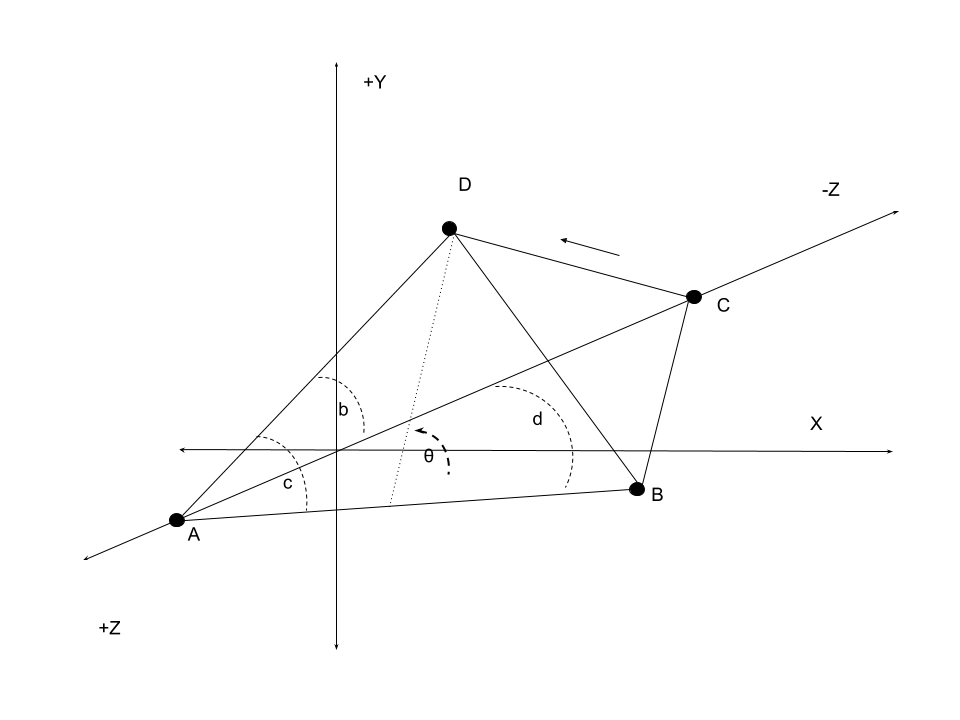
\includegraphics[width=0.70\textwidth]{figures/EasyToComputeTetDerivative.png}
     \caption{Basic diagram of initial tetrahedron}
  \label{fig:basic}     
\end{figure}

This method computes the dihedral angles from the vertex angls. Let $\angle b, \angle c,\angle d$ be the
vertx angles of the triangles $\Delta ACD, \Delta ABD, \Delta ABC$ meeting in a point (angles being named after the opposing edged).
($\angle AB$ is a dihedral angle), and $b,c,d$ are planar angles against the vertex of the
tetrahedron.

\begin{equation}
  \label{dihedral}
 \angle AB =\arccos{\frac{\cos{b} - \cos{c}\cos{d}}{\sin{c}\sin{d}}}
\end{equation}

When moving one edge $CD$ of a tetrahedron $ABCD$ assuming $A,B$ and $C$ are fixed, we are most interested in the change of
the dihedral angle $\angle \theta = \angle AB$ opposite the edge $CD$. This can be computed as the derivative of the angle $\angle AB$
with respect to the change in a single vertex angle $b$, which changes as the length $CD$
changes. Because $D$ is on a fixed hinge rotating about $AB$, The change in the postion of $D$ is a function of the change in
the angle $\angle AB$.

By the chain rule,

\begin{equation}
\frac{\partial \theta }{\partial \overline{DC}}   =  \frac{\partial \angle AB }{\partial b} \frac{\partial b}{\partial \overline{DC}} 
\end{equation}

By differentiation \ref{dihedral} with respect to $b$, we obtain:
\begin{equation}
\frac{\partial \angle AB }{\partial b} =
\frac{\csc{c} \csc{d} \sin{b}}
 {\sqrt{1 - \csc^2{c} \csc^2{d} \big( \cos{b} - \cos{c} \cos{d}\big)^2}}
\end{equation}

Via cosine law, let $x = \overline{AC}, y = \overline{AD}, z = \overline{CD}$,
\[
b = \arccos{\frac{x^2 + y^2 + -z^2}{2xy}}
\]

\[
\frac{\partial b}{\partial \overline{DC}} = \frac{z}{x y \sqrt{1 -
    \frac{(x^2 + y^2 - z^2)^2}{(4 x^2 y^2)}}}
\]


If we have a goal node $g$ which exists further down the kinematic chain than $\overline{DC}$, then
the change in its position can be computed as the rotation of it about $\overline{AB}$ induced by the
chage in length $\overline{DC}$.

\begin{equation}
\frac{\partial \angle AB }{\partial \overline{DC}}  =
\frac{z}{x y \sqrt{1 -
    \frac{(x^2 + y^2 - z^2)^2}{(4 x^2 y^2)}}}
\cdot
\frac{\csc{c} \csc{d} \sin{b}}
 {\sqrt{1 - \csc^2{c} \csc^2{d} \big( \cos{b} - \cos{c} \cos{d}\big)^2}}
\end{equation}

 Note that the change in position of a goal point $G$ rotated about $\overrightarrow{AB}$ is:

 (from \url{http://reedbeta.com/blog/rotations-and-infinitesimal-generators/}:)

 Because the triangle $\Delta BCD$ is changing, an object attached a space frame attached to $\Delta BCD$ moves in a complex way.
 However, $\Delta ABD$ is not changed by a change to $\overline{DC}$, so if there was an object rigidly attached to the triangular face $\Delta ABD$ at postion $G$ (and in, particular it is possible that $G = D$,
then its change in positions would be given by:

\begin{equation}
\frac{\partial \overrightarrow{G}}{\partial \angle AB} = \overrightarrow{AB} \times \overrightarrow{BG}
\end{equation}

so:
\begin{equation}
\frac{\partial \overrightarrow{G}}{\partial \overline{DC}} =  \frac{\partial \overrightarrow{G}}{\partial \angle AB } \frac{\partial \angle AB }{\partial \overline{DC}} = (\overrightarrow{AB} \times \overrightarrow{BG}) \cdot \frac{\partial \angle AB }{\partial \overline{DC}}
\end{equation}

By assigning $G = D$, we now have an analytic calculation of $\frac{\partial D}{\partial \overline{DC}}$.

\subsection{The change in addtional nodes}

Assuming that $A, B$, and $C$ are fixed, the computation of motion of $D,E$, and $F$ as the length $ \overline{DC} $ changes is interesting
because each is in a sense different. If we had a formula for each of these, they would all be different.

However, nodes further away from $\overline{CD}$, that is, those that would be numbered $H$ and above, have a uniformity because changing
$\overline{CD}$ changes the orientation and position, but not the shape, of the triangle $\Delta D, E, F$. Therefore, every point fixed
to this triangle can modeled as a change to this fixed frames. Therefore, to compute the change in the position of any point attached beyond
nodes $\Delta D, E, F$ can be calculated simply from the change to $D,E$ and $F$.

It is therefore advantageous to be able to efficiently and clearly caclulate
$\frac{\partial D}{\partial \overline{DC}}$,
$\frac{\partial E}{\partial \overline{DC}}$ and
$\frac{\partial F}{\partial \overline{DC}}$.

If we cannot produce closed-form expressions for these derivatives, we need to be able to approximate them well via differentials.

The motion of $E$ is a pure rotation about the fixed nodes $B$ and $E$. We will have no such luck with $F$ and $G$.

Similar to our deriviation of the motion of $D$, we compute the motion of $E$ by finding the change to the angle $\psi$ around the
vector $\overrightarrow{CB}$. We compute this change in motion by differentiating the formula for the dihedral angle $\angle BC$ of
the tetrahedron $BCDE$ from the apex $C$:

\begin{equation}
 \angle BC  =\arccos{\frac{\cos{\angle DCE} - \cos{\angle BCD}\cos{\angle BCE}}{\sin{\angle BCD}\sin{\angle BCE}}}
\end{equation}

The angle $\angle BCE$ does not change as $CD$ changes its length. The angles $\angle BCD$ and $\angle DCE$ do both
change their length in response to a change to $\overline{CD}$, so we rewrite this formula in terms of that to facilitate differentiation.

\begin{equation}
\angle BCD  = \arccos{\frac{\overline{BC}^2 + \overline{CD}^2 + -\overline{BD}^2}{2\overline{BC}\cdot\overline{CD}}}
\end{equation}

% arccos((r^2 + z^2 - t^2)/(2*r*z)

\begin{equation}
\angle DCE  = \arccos{\frac{\overline{CD}^2 + \overline{CE}^2 + -\overline{DE}^2}{2\overline{CD}\cdot \overline{CE}}}
\end{equation}

% arccos((z^2 + q^2 - t^2)/(2*q*z)

Via cosine law, let $x = \overline{AC}, y = \overline{AD}, z = \overline{CD}, r = \overline{BC}, s = \overline{ED},
t = \overline{BD}, q = \overline{CE},$

\begin{align*}
  f(z) =  & \frac{z^2 + q^2 + -s^2}{2z\cdot q} \\
  f'(z) = & \frac{-q^2 + s^2 + z^2}{2 q z^2}
\end{align*}

\begin{align*}
  g(z) = &  \frac{r^2 + z^2 + -t^2}{2r\cdot z} \\
  g'(z) = & \frac{-r^2 + t^2 + z^2}{2 r z^2}
\end{align*}

\begin{equation}
  \frac{\partial \angle BC}{\partial z} =
  \frac{\partial }{\partial z} \arccos{\frac{f(z) - g(z)\cos{\angle BCE}}{\sin{\arccos{g(z)}}\sin{\angle BCE}}}
\end{equation}

Let: $a = \angle BCE$.

\begin{equation}
  \frac{\partial \angle BC}{\partial z} =
  -\frac{\frac{\sin{a} (f'(z) - \cos{a} g'(z))}{\sqrt{1 - g(z)^2}} + \frac{\sin{a} g(z) g'(z) (f(z) - \cos{a} g(z))}{(1 - g(z)^2)^(3/2)}}
{\sqrt{1 - \frac{\sin^2{a} (f(z) - \cos{a} g(z))^2}{1 - g(z)^2}}}
\end{equation}


As we did before, any point $M$ attached rigidely to the triange $\Delta BCE$ is  computable via the expression:
\begin{equation}
  \frac{\partial M}{\partial \overline{CD}} = \overrightarrow{CE} \times \overrightarrow{CB}
  \frac{\partial \angle BC}{\partial \overline{CD}}
  \end{equation}

In order to discuss goal nodes greater than $D$ as $\overline{CD}$ changes, recall that $E$ is attached as tetrahedron $BCDE$ to nodes $B, C$ and $D$
with joints allowing angular displacement. 


 It is important to note that this expression in terms of the tetrahedron $ABCD$ belie the rather tricky coding
 involved. The code must be very careful to consider the chirality of the tetrahedron, in particular, and
 the choice of the points $ABCD$ must be done carefully. In fact, my code, perhaps incompetently, choose the points $A$ and $B$
 by swapping them if the tetrarhedron $ABCD$ is not anticlockwise (that is, $D$ is on the righ-hand side (right thumb pointing to it),
 when the fingers rotate from $A$ to $B$ to $C$.)

 Furthermore, I actually return the derivative in a ``normalized'' form. I am not sure that is justified, but it seems to work with the
 DLIB software. In theory we should be quite able to say what the units of these derivatibves are, but I get rather confused by them.
 
Let's assume however that we have a way to compute the $\frac{\partial g}{\partial \overline{DC}}$. Have we then got a way to compute
the change in the score value?

However, in order to use the DLIB numerical optimization software, what we really need to compute is
an objective function and the change in this objective function as we change lengths within the system.
Our basic goal is minimize an objective function $S$ which represents the sum of the distances between the
goal node positions $C(g)$  and their target positions $T(g)$.

\[
S(C) = \sum_{g\in V} \| C(g) - T(g) \|
\]

The change in the components of this sum are captured by the inner product of the derivative with the vector
pointing from the current node position $C(g)$ to the target $T(g)$.

Our goal is to compute the change in this function with respect to the change in the length of a given edge:

\[
\frac{\partial S}{\partial \overline{DC}} =
\sum_{g\in V} [C(g) - T(g)] \cdot \frac{\partial AB }{\partial \overline{DC}} 
\]

Note that $[C(g) - T(g)]$ points {\em away} from the goal. This because we have organized our system to {\em minimize} the objective $S$,
as is customary.




\section{Unvetted References}

A starting point is: \cite{Hanahara2008}.

This paper use gradient computation in a hybrid approach:

\url{http://ieeexplore.ieee.org/stamp/stamp.jsp?tp=&arnumber=478427}

It very explicitly uses ``backbone curve'' and then fits manipulators to it.
This says :  ``In fact, the need to derive expressions for these
derivatives for the parallelherial structures often used in real
hyper-redundant systems is a major drawback of the Jacobian
based methods.''

However, in the case of this statically determinate VGTs it doesn't seem to bad.

This article is interesting:

Kinematic transformations for remotely-actuated planar continuum robots

I really need to read this:

``Tetrahedral Robotics for Space Exploration''

Need to understand this:

Cite this chapter as:
Gilbert H.B., Rucker D.C., Webster III R.J. (2016) Concentric Tube Robots: The State of the Art and Future Directions. In: Inaba M., Corke P. (eds) Robotics Research. Springer Tracts in Advanced Robotics, vol 114. Springer, Cham

This article: needs to be read and thoroughly understood:

\url{http://ieeexplore.ieee.org/document/999655/}

\url{https://digitalscholarship.unlv.edu/cgi/viewcontent.cgi?article=2259&context=thesesdissertations}

\bibliographystyle{unsrt}
\bibliography{vgt}


\end{document}

http://eprints.cs.vt.edu/archive/00000192/01/TR-90-10.pdf


https://people.eecs.berkeley.edu/~elghaoui/Teaching/EE227A/lecture6.pdf

http://homes.cs.washington.edu/~sagarwal/aat.pdf

http://zoonek.free.fr/blosxom/R/2012-06-01_Optimization.html

http://docs.mosek.com/modeling-cookbook/cqo.html

// This one looks pretty interesting
http://ieeexplore.ieee.org/abstract/document/4160811/

https://tspace.library.utoronto.ca/bitstream/1807/14046/1/NQ49815.pdf



